 
%% bare_conf_compsoc.tex
%% V1.4b
%% 2015/08/26
%% by Michael Shell
%% See:
%% http://www.michaelshell.org/
%% for current contact information.
%%
%% This is a skeleton file demonstrating the use of IEEEtran.cls
%% (requires IEEEtran.cls version 1.8b or later) with an IEEE Computer
%% Society conference paper.
%%
%% Support sites:
%% http://www.michaelshell.org/tex/ieeetran/
%% http://www.ctan.org/pkg/ieeetran
%% and
%% http://www.ieee.org/

%%*************************************************************************
%% Legal Notice:
%% This code is offered as-is without any warranty either expressed or
%% implied; without even the implied warranty of MERCHANTABILITY or
%% FITNESS FOR A PARTICULAR PURPOSE! 
%% User assumes all risk.
%% In no event shall the IEEE or any contributor to this code be liable for
%% any damages or losses, including, but not limited to, incidental,
%% consequential, or any other damages, resulting from the use or misuse
%% of any information contained here.
%%
%% All comments are the opinions of their respective authors and are not
%% necessarily endorsed by the IEEE.
%%
%% This work is distributed under the LaTeX Project Public License (LPPL)
%% ( http://www.latex-project.org/ ) version 1.3, and may be freely used,
%% distributed and modified. A copy of the LPPL, version 1.3, is included
%% in the base LaTeX documentation of all distributions of LaTeX released
%% 2003/12/01 or later.
%% Retain all contribution notices and credits.
%% ** Modified files should be clearly indicated as such, including  **
%% ** renaming them and changing author support contact information. **
%%*************************************************************************


% *** Authors should verify (and, if needed, correct) their LaTeX system  ***
% *** with the testflow diagnostic prior to trusting their LaTeX platform ***
% *** with production work. The IEEE's font choices and paper sizes can   ***
% *** trigger bugs that do not appear when using other class files.       ***                          ***
% The testflow support page is at:
% http://www.michaelshell.org/tex/testflow/



\documentclass[journal,compsoc]{IEEEtran}
% Some/most Computer Society conferences require the compsoc mode option,
% but others may want the standard conference format.
%
% If IEEEtran.cls has not been installed into the LaTeX system files,
% manually specify the path to it like:
% \documentclass[conference,compsoc]{../sty/IEEEtran}





% Some very useful LaTeX packages include:
% (uncomment the ones you want to load)


% *** MISC UTILITY PACKAGES ***
%
%\usepackage{ifpdf}
% Heiko Oberdiek's ifpdf.sty is very useful if you need conditional
% compilation based on whether the output is pdf or dvi.
% usage:
% \ifpdf
%   % pdf code
% \else
%   % dvi code
% \fi
% The latest version of ifpdf.sty can be obtained from:
% http://www.ctan.org/pkg/ifpdf
% Also, note that IEEEtran.cls V1.7 and later provides a builtin
% \ifCLASSINFOpdf conditional that works the same way.
% When switching from latex to pdflatex and vice-versa, the compiler may
% have to be run twice to clear warning/error messages.






% *** CITATION PACKAGES ***
%
\ifCLASSOPTIONcompsoc
  % IEEE Computer Society needs nocompress option
  % requires cite.sty v4.0 or later (November 2003)
  \usepackage[nocompress]{cite}
\else
  % normal IEEE
  \usepackage{cite}
\fi
% cite.sty was written by Donald Arseneau
% V1.6 and later of IEEEtran pre-defines the format of the cite.sty package
% \cite{} output to follow that of the IEEE. Loading the cite package will
% result in citation numbers being automatically sorted and properly
% "compressed/ranged". e.g., [1], [9], [2], [7], [5], [6] without using
% cite.sty will become [1], [2], [5]--[7], [9] using cite.sty. cite.sty's
% \cite will automatically add leading space, if needed. Use cite.sty's
% noadjust option (cite.sty V3.8 and later) if you want to turn this off
% such as if a citation ever needs to be enclosed in parenthesis.
% cite.sty is already installed on most LaTeX systems. Be sure and use
% version 5.0 (2009-03-20) and later if using hyperref.sty.
% The latest version can be obtained at:
% http://www.ctan.org/pkg/cite
% The documentation is contained in the cite.sty file itself.
%
% Note that some packages require special options to format as the Computer
% Society requires. In particular, Computer Society  papers do not use
% compressed citation ranges as is done in typical IEEE papers
% (e.g., [1]-[4]). Instead, they list every citation separately in order
% (e.g., [1], [2], [3], [4]). To get the latter we need to load the cite
% package with the nocompress option which is supported by cite.sty v4.0
% and later.





% *** GRAPHICS RELATED PACKAGES ***
%
\ifCLASSINFOpdf
  % \usepackage[pdftex]{graphicx}
  % declare the path(s) where your graphic files are
  % \graphicspath{{../pdf/}{../jpeg/}}
  % and their extensions so you won't have to specify these with
  % every instance of \includegraphics
  % \DeclareGraphicsExtensions{.pdf,.jpeg,.png}
\else
  % or other class option (dvipsone, dvipdf, if not using dvips). graphicx
  % will default to the driver specified in the system graphics.cfg if no
  % driver is specified.
  % \usepackage[dvips]{graphicx}
  % declare the path(s) where your graphic files are
  % \graphicspath{{../eps/}}
  % and their extensions so you won't have to specify these with
  % every instance of \includegraphics
  % \DeclareGraphicsExtensions{.eps}
\fi
% graphicx was written by David Carlisle and Sebastian Rahtz. It is
% required if you want graphics, photos, etc. graphicx.sty is already
% installed on most LaTeX systems. The latest version and documentation
% can be obtained at: 
% http://www.ctan.org/pkg/graphicx
% Another good source of documentation is "Using Imported Graphics in
% LaTeX2e" by Keith Reckdahl which can be found at:
% http://www.ctan.org/pkg/epslatex
%
% latex, and pdflatex in dvi mode, support graphics in encapsulated
% postscript (.eps) format. pdflatex in pdf mode supports graphics
% in .pdf, .jpeg, .png and .mps (metapost) formats. Users should ensure
% that all non-photo figures use a vector format (.eps, .pdf, .mps) and
% not a bitmapped formats (.jpeg, .png). The IEEE frowns on bitmapped formats
% which can result in "jaggedy"/blurry rendering of lines and letters as
% well as large increases in file sizes.
%
% You can find documentation about the pdfTeX application at:
% http://www.tug.org/applications/pdftex





% *** MATH PACKAGES ***
%
%\usepackage{amsmath}
% A popular package from the American Mathematical Society that provides
% many useful and powerful commands for dealing with mathematics.
%
% Note that the amsmath package sets \interdisplaylinepenalty to 10000
% thus preventing page breaks from occurring within multiline equations. Use:
%\interdisplaylinepenalty=2500
% after loading amsmath to restore such page breaks as IEEEtran.cls normally
% does. amsmath.sty is already installed on most LaTeX systems. The latest
% version and documentation can be obtained at:
% http://www.ctan.org/pkg/amsmath





% *** SPECIALIZED LIST PACKAGES ***
%
%\usepackage{algorithmic}
% algorithmic.sty was written by Peter Williams and Rogerio Brito.
% This package provides an algorithmic environment fo describing algorithms.
% You can use the algorithmic environment in-text or within a figure
% environment to provide for a floating algorithm. Do NOT use the algorithm
% floating environment provided by algorithm.sty (by the same authors) or
% algorithm2e.sty (by Christophe Fiorio) as the IEEE does not use dedicated
% algorithm float types and packages that provide these will not provide
% correct IEEE style captions. The latest version and documentation of
% algorithmic.sty can be obtained at:
% http://www.ctan.org/pkg/algorithms
% Also of interest may be the (relatively newer and more customizable)
% algorithmicx.sty package by Szasz Janos:
% http://www.ctan.org/pkg/algorithmicx




% *** ALIGNMENT PACKAGES ***
%
%\usepackage{array}
% Frank Mittelbach's and David Carlisle's array.sty patches and improves
% the standard LaTeX2e array and tabular environments to provide better
% appearance and additional user controls. As the default LaTeX2e table
% generation code is lacking to the point of almost being broken with
% respect to the quality of the end results, all users are strongly
% advised to use an enhanced (at the very least that provided by array.sty)
% set of table tools. array.sty is already installed on most systems. The
% latest version and documentation can be obtained at:
% http://www.ctan.org/pkg/array


% IEEEtran contains the IEEEeqnarray family of commands that can be used to
% generate multiline equations as well as matrices, tables, etc., of high
% quality.




% *** SUBFIGURE PACKAGES ***
%\ifCLASSOPTIONcompsoc
%  \usepackage[caption=false,font=footnotesize,labelfont=sf,textfont=sf]{subfig}
%\else
%  \usepackage[caption=false,font=footnotesize]{subfig}
%\fi
% subfig.sty, written by Steven Douglas Cochran, is the modern replacement
% for subfigure.sty, the latter of which is no longer maintained and is
% incompatible with some LaTeX packages including fixltx2e. However,
% subfig.sty requires and automatically loads Axel Sommerfeldt's caption.sty
% which will override IEEEtran.cls' handling of captions and this will result
% in non-IEEE style figure/table captions. To prevent this problem, be sure
% and invoke subfig.sty's "caption=false" package option (available since
% subfig.sty version 1.3, 2005/06/28) as this is will preserve IEEEtran.cls
% handling of captions.
% Note that the Computer Society format requires a sans serif font rather
% than the serif font used in traditional IEEE formatting and thus the need
% to invoke different subfig.sty package options depending on whether
% compsoc mode has been enabled.
%
% The latest version and documentation of subfig.sty can be obtained at:
% http://www.ctan.org/pkg/subfig




% *** FLOAT PACKAGES ***
%
%\usepackage{fixltx2e}
% fixltx2e, the successor to the earlier fix2col.sty, was written by
% Frank Mittelbach and David Carlisle. This package corrects a few problems
% in the LaTeX2e kernel, the most notable of which is that in current
% LaTeX2e releases, the ordering of single and double column floats is not
% guaranteed to be preserved. Thus, an unpatched LaTeX2e can allow a
% single column figure to be placed prior to an earlier double column
% figure.
% Be aware that LaTeX2e kernels dated 2015 and later have fixltx2e.sty's
% corrections already built into the system in which case a warning will
% be issued if an attempt is made to load fixltx2e.sty as it is no longer
% needed.
% The latest version and documentation can be found at:
% http://www.ctan.org/pkg/fixltx2e


%\usepackage{stfloats}
% stfloats.sty was written by Sigitas Tolusis. This package gives LaTeX2e
% the ability to do double column floats at the bottom of the page as well
% as the top. (e.g., "\begin{figure*}[!b]" is not normally possible in
% LaTeX2e). It also provides a command:
%\fnbelowfloat
% to enable the placement of footnotes below bottom floats (the standard
% LaTeX2e kernel puts them above bottom floats). This is an invasive package
% which rewrites many portions of the LaTeX2e float routines. It may not work
% with other packages that modify the LaTeX2e float routines. The latest
% version and documentation can be obtained at:
% http://www.ctan.org/pkg/stfloats
% Do not use the stfloats baselinefloat ability as the IEEE does not allow
% \baselineskip to stretch. Authors submitting work to the IEEE should note
% that the IEEE rarely uses double column equations and that authors should try
% to avoid such use. Do not be tempted to use the cuted.sty or midfloat.sty
% packages (also by Sigitas Tolusis) as the IEEE does not format its papers in
% such ways.
% Do not attempt to use stfloats with fixltx2e as they are incompatible.
% Instead, use Morten Hogholm'a dblfloatfix which combines the features
% of both fixltx2e and stfloats:
%
% \usepackage{dblfloatfix}
% The latest version can be found at:
% http://www.ctan.org/pkg/dblfloatfix




% *** PDF, URL AND HYPERLINK PACKAGES ***
%
%\usepackage{url}
% url.sty was written by Donald Arseneau. It provides better support for
% handling and breaking URLs. url.sty is already installed on most LaTeX
% systems. The latest version and documentation can be obtained at:
% http://www.ctan.org/pkg/url
% Basically, \url{my_url_here}.




% *** Do not adjust lengths that control margins, column widths, etc. ***
% *** Do not use packages that alter fonts (such as pslatex).         ***
% There should be no need to do such things with IEEEtran.cls V1.6 and later.
% (Unless specifically asked to do so by the journal or conference you plan
% to submit to, of course. )


% correct bad hyphenation here
\hyphenation{op-tical net-works semi-conduc-tor}

\usepackage{graphicx}
\graphicspath{{figures/}}

\begin{document}
%
% paper title
% Titles are generally capitalized except for words such as a, an, and, as,
% at, but, by, for, in, nor, of, on, or, the, to and up, which are usually
% not capitalized unless they are the first or last word of the title.
% Linebreaks \\ can be used within to get better formatting as desired.
% Do not put math or special symbols in the title.
\title{Machine Learning for Automated Diagnosis of Skin Lesions}


% author names and affiliations
% use a multiple column layout for up to three different
% affiliations
\author{\IEEEauthorblockN{Fábio Santos}
\IEEEauthorblockA{Department of Electronics\\Telecomunications and Informatics\\
University of Aveiro\\
Aveiro, 3810-193\\
Email: fmts@ua.pt}
}

% conference papers do not typically use \thanks and this command
% is locked out in conference mode. If really needed, such as for
% the acknowledgment of grants, issue a \IEEEoverridecommandlockouts
% after \documentclass

% for over three affiliations, or if they all won't fit within the width
% of the page (and note that there is less available width in this regard for
% compsoc conferences compared to traditional conferences), use this
% alternative format:
% 
%\author{\IEEEauthorblockN{Michael Shell\IEEEauthorrefmark{1},
%Homer Simpson\IEEEauthorrefmark{2},
%James Kirk\IEEEauthorrefmark{3}, 
%Montgomery Scott\IEEEauthorrefmark{3} and
%Eldon Tyrell\IEEEauthorrefmark{4}}
%\IEEEauthorblockA{\IEEEauthorrefmark{1}School of Electrical and Computer Engineering\\
%Georgia Institute of Technology,
%Atlanta, Georgia 30332--0250\\ Email: see http://www.michaelshell.org/contact.html}
%\IEEEauthorblockA{\IEEEauthorrefmark{2}Twentieth Century Fox, Springfield, USA\\
%Email: homer@thesimpsons.com}
%\IEEEauthorblockA{\IEEEauthorrefmark{3}Starfleet Academy, San Francisco, California 96678-2391\\
%Telephone: (800) 555--1212, Fax: (888) 555--1212}
%\IEEEauthorblockA{\IEEEauthorrefmark{4}Tyrell Inc., 123 Replicant Street, Los Angeles, California 90210--4321}}




% use for special paper notices
%\IEEEspecialpapernotice{(Invited Paper)}




% make the title area
\maketitle

% As a general rule, do not put math, special symbols or citations
% in the abstract
\begin{abstract}
Machine learning, specifically, deep learning is a fast-growing field in medicine which is being used for multiple medical imaging related problems, such as early detection of skin cancer. Even though, such systems don't lay out a 100\% accurate diagnostic they aim to provide support for both dermatologists in the decision making process and for patients that don’t have access to skin professionals.  
In this paper we will focus on the current state of skin cancer recognition using CNN’s (Convolutional Neural Networks) and on skin cancer recognition applications for dermatology decision support. We aim to integrate these concepts into real world use by demonstrating how these systems have potential to change the landscape of medical imaging. 
\end{abstract}

% no keywords




% For peer review papers, you can put extra information on the cover
% page as needed:
% \ifCLASSOPTIONpeerreview
% \begin{center} \bfseries EDICS Category: 3-BBND \end{center}
% \fi
%
% For peerreview papers, this IEEEtran command inserts a page break and
% creates the second title. It will be ignored for other modes.
\IEEEpeerreviewmaketitle

\section{Introduction}
\subsection{Background}
Skin cancer is the most common cancer in the United States and worldwide, particularly, in America 1 in 5 persons will develop skin cancer by the age of 70 \cite{Foundation2019}. However, skin cancer represents a international problem for the health community. For instance, in Europe, over 100,000 people are diagnosed with melanoma and 22,000  deaths are caused by this form of skin cancer annually \cite{Bray2018}.  But the most interesting fact about skin cancer is that when detected early, the 5-year survival rate for melanoma is 99 percent, as opposed to 23 predicted percent rate from late stages \cite{Foundation2019}. \par
Initially, automated diagnosis of skin lesions was made based on predefined techniques well known by dermatology professionals, but often failed to either generalize to new cases or lacked the accuracy of a human. However in more recent years, a lot of work has put into medical applications of machine learning. The reason behind this shift are technical, namely: \par
\begin{itemize}
\item Huge amounts of data collected over the years, specifically, labelled skin cancer images
\item Exponential computing power growth over the years 
\item Deep learning algorithm research
\end{itemize}
Contrary to other traditional machine learning algorithms, deep learning removes the need for feature engineering, which is a quite time consuming process which is both difficult to do and can introduce human error. In addition, it is relatively easy to adapt or modify existing deep learning architectures on new applications.
\subsection{Objectives and Motivation}
The main objective behind this work is to improve the current work on deep learning techniques through CNN's and to develop a production ready application which enables easy communication between patients and dermatologists.
\begin{figure}[h]
  \centering
    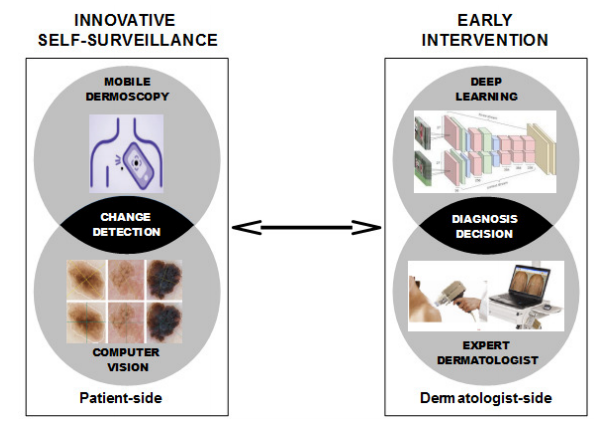
\includegraphics[scale=0.5, width=\linewidth]{figures/Dissertation_Plan.png}
  \caption{Dissertation Work Plan}
\end{figure}
The first version of this application should be able to allow image sharing between patients and dermatologists as well as provide a deep learning based decision support tool for dermatologists. Because this tool has the intent of being production ready, it is highly important to improve the deep learning algorithm as much as possible to the point that it becomes comparable to a dermatologist in terms of accuracy. \par 
An important consideration for this work is to design an architecture which allows for future expansion of the system, for example for providing new features such as a self surveillance change detection which would allow users to monitor their own lesions.  
\section{Literature review}
\subsection{eHealth and mHealth applications}
The emergence of eHealth/mHealth applications presents exciting opportunities to enhance clinical care, health promotion, and disease prevention. However, it can be quite a challenge for professionals to adapt to these systems and integrate them into the clinical workflow, particularly, to seek guidance for decision making.
\subsection{Deep neural networks}
Deep learning algorithms are providing exciting solutions for medical image analysis problems and they are seen as a key method for future applications. The initial impact of deep learning for medical imaging was revealed through a special issue published in the IEEE Transactions on Medical Imaging (Greenspan, Ginneken and Summers, 2016).
The surveys by Hu et al., (2018) and Litjens et al. (2017) contributes also to a clear understanding of the principles and methods of neural network and deep learning concepts, showing how the algorithms based on deep models are being applied to medical image in a wide variety of application areas.
The successes of deep learning architectures such as deep neural networks (DNNs), deep belief networks (DBNs) and recurrent neural networks (RNNs) are now well reported in the areas of computer vision, speech recognition, natural language processing and gaming. A comprehensive and up to date approach to deep learning can be found elsewhere (Goodfellow, Bengio and Courville, 2016; LeCun, Bengio and Hinton, 2015). 
\subsection{Skin lesion classification using deep learning}
The first Deep Convulutional Neural Network (a type of deep  network) for skin cancer classification was first introduced in 2017 by Esteva et al.\cite{Esteva2017}, which classified keratinocyte cancer and melanoma. The authors follow a transfer learning approach by leveraging the weights of the InceptionV3 network trained on ImageNet, on top of which they build their own classifier. Finally, they measured the network's performance by pitting it against 21 dermatologists that resulted in comparable accuracy to that of those board-certified dermatologists. This network used a very large set of labelled images in order to achieve high accuracy, namely, 129 450 clinical images (including 3374 dermoscopic images) \cite{Esteva2017}. This data was a combination of biopsy proven datasets from Edinburgh Dermofit Library, Stanford Hospital and from a initiative called ISIC. \par
\subsubsection{International Skin Imaging Collaboration (ISIC)}
One of the most important factors which determines a network's performance is the dataset used to train it on. Several public datasets such as ImageNet are quite useful to create generic models, however, for skin lesion classification datasets such as the BCN\_20000\cite{bcn_20000} are used. \par
Unfortunately, it is difficult and in many times impossible to compare the performance of published classification results since many authors use nonpublic datasets for training and/or testing \cite{Brinker2018}. Despite this, the HAM10000 dataset is the closest we have to a benchmark dataset for testing deep networks currently available and therefore we should use it to test ours \cite{ham10000}. \par
International Skin Imaging Collaboration (ISIC) arose from the need for an open source public access archive of skin images and are trying. This archive serves as a public resource of images for teaching and for the development and testing of automated diagnostic systems and every year places a challenge around their datasets \cite{isic2019}. \par
In part 3 of the ISIC 2018 challenge participants were asked to develop a classifier to distinguish between 7 different types of skin cancer. The provided dataset for the challenge was the HAM10000 but participants could complement that dataset by gathering their own. Finally, participant's were ranked based on their normalized multiclass accuracy (accuracy of the classifier on each of the classes averaged together) \cite{isic2018}. The top 3 submissions had balanced accuracies of about 0.885, 0.882, 0.871 respectively and were all submited by a company called Metaoptima \cite{isic2018top3}, which as we will see later has products related to skin lesion classification on production environments. To train those networks they used the competition’s HAM10000 dataset along with the ISIC Archive and other proprietary data. Additionally, they augmented the training data by performing random horizontal flips, random rotations, changes in brightness, saturation, and contrast. They used a method called transfer learning (which we will describe later in more detail) from several models trained on ImageNet (such as InceptionV3 or ResNet-50), and then choosed the best-performing and ensembled them together \cite{isic2018top3}. \par
The 2019's version of this challenge asked participants to classify dermoscopic images among nine different diagnostic categories such as "melanoma" or "dermatofibroma", however this time around one of the classes was unkown (none of the others). Similarly to the 2018's version participants could use their own data to improve the network's performance and were ranked based on a balanced multiclass accuracy \cite{isic2019}. 
The results turned out to be quite promising, with the best submission posted by Geesert et al. \cite{isic2019first} scoring 92.6\% accuracy. They trained their networks on the HAM10000, \cite{ham10000}, BCN\_20000 \cite{bcn_20000} and MSK \cite{msk} datasets. The following points represent their training process:  
\begin{itemize}
\item Preprocessing methods such as cropping are applied based on the mean intensity differential between the mole area and the non mole area, they binarize the images, apply the shades of gray color constancy method (just like the 2018's top 3) and finally resize the larger images in the datasets. 
\item Data augmentation is performed by randomly changing brightness, contrast, rotation, scale, shear and flip.
\item Two different input strategies are used. While the first takes a random crop from the preprocessed image, the second randomly resizes and scales the image when taking a crop from the preprocessed one.
\item They use a transfer learning based approach relying on EfficientNets that were trained on the ImageNet dataset. For each model predictions are made based which input strategies was used. 
\item Finally, they find the optimal subset of models and ensemble them together
\end{itemize}
\subsection{Teldermathology and deep learning}
Because of the visual nature of a skin examination, teledermatology has the potential to become a powerful tool in the diagnosis and management of skin diseases, especially in rural areas where specialty services may not be available. 
Currently, several production ready skin lesion classification systems are currently available for both skin professionals and patients wishing to self monitor skin moles. However, almost none of them has shown to be sufficiently accurate and/or reliable enough for a clinical environment. \par 
One of the most popular applications for this purpose is Metaoptima's Dermengine web application. Their Visual Search tool compares a user-submitted image with similar images in a database of thousands of pathology-labelled images gathered from expert dermatologists around the world. Deep learning techniques are used to search for related images based on visual features such as colour, shape, and patterns \cite{dermengine}. \par
% An example of a floating figure using the graphicx package.
% Note that \label must occur AFTER (or within) \caption.
% For figures, \caption should occur after the \includegraphics.
% Note that IEEEtran v1.7 and later has special internal code that
% is designed to preserve the operation of \label within \caption
% even when the captionsoff option is in effect. However, because
% of issues like this, it may be the safest practice to put all your
% \label just after \caption rather than within \caption{}.
%
% Reminder: the "draftcls" or "draftclsnofoot", not "draft", class
% option should be used if it is desired that the figures are to be
% displayed while in draft mode.
%
%\begin{figure}[!t]
%\centering
%\includegraphics[width=2.5in]{myfigure}
% where an .eps filename suffix will be assumed under latex, 
% and a .pdf suffix will be assumed for pdflatex; or what has been declared
% via \DeclareGraphicsExtensions.
%\caption{Simulation results for the network.}
%\label{fig_sim}
%\end{figure}

% Note that the IEEE typically puts floats only at the top, even when this
% results in a large percentage of a column being occupied by floats.


% An example of a double column floating figure using two subfigures.
% (The subfig.sty package must be loaded for this to work.)
% The subfigure \label commands are set within each subfloat command,
% and the \label for the overall figure must come after \caption.
% \hfil is used as a separator to get equal spacing.
% Watch out that the combined width of all the subfigures on a 
% line do not exceed the text width or a line break will occur.
%
%\begin{figure*}[!t]
%\centering
%\subfloat[Case I]{\includegraphics[width=2.5in]{box}%
%\label{fig_first_case}}
%\hfil
%\subfloat[Case II]{\includegraphics[width=2.5in]{box}%
%\label{fig_second_case}}
%\caption{Simulation results for the network.}
%\label{fig_sim}
%\end{figure*}
%
% Note that often IEEE papers with subfigures do not employ subfigure
% captions (using the optional argument to \subfloat[]), but instead will
% reference/describe all of them (a), (b), etc., within the main caption.
% Be aware that for subfig.sty to generate the (a), (b), etc., subfigure
% labels, the optional argument to \subfloat must be present. If a
% subcaption is not desired, just leave its contents blank,
% e.g., \subfloat[].


% An example of a floating table. Note that, for IEEE style tables, the
% \caption command should come BEFORE the table and, given that table
% captions serve much like titles, are usually capitalized except for words
% such as a, an, and, as, at, but, by, for, in, nor, of, on, or, the, to
% and up, which are usually not capitalized unless they are the first or
% last word of the caption. Table text will default to \footnotesize as
% the IEEE normally uses this smaller font for tables.
% The \label must come after \caption as always.
%
%\begin{table}[!t]
%% increase table row spacing, adjust to taste
%\renewcommand{\arraystretch}{1.3}
% if using array.sty, it might be a good idea to tweak the value of
% \extrarowheight as needed to properly center the text within the cells
%\caption{An Example of a Table}
%\label{table_example}
%\centering
%% Some packages, such as MDW tools, offer better commands for making tables
%% than the plain LaTeX2e tabular which is used here.
%\begin{tabular}{|c||c|}
%\hline
%One & Two\\
%\hline
%Three & Four\\
%\hline
%\end{tabular}
%\end{table}


% Note that the IEEE does not put floats in the very first column
% - or typically anywhere on the first page for that matter. Also,
% in-text middle ("here") positioning is typically not used, but it
% is allowed and encouraged for Computer Society conferences (but
% not Computer Society journals). Most IEEE journals/conferences use
% top floats exclusively. 
% Note that, LaTeX2e, unlike IEEE journals/conferences, places
% footnotes above bottom floats. This can be corrected via the
% \fnbelowfloat command of the stfloats package.


\section{Methods}
\subsection{Artifitial neural networks (ANN's)}
Artificial Neural Networks (also known as ANNs) compose a category of machine learning algorithms which are inspired by biological neural networks from either humans or animals alike.
\begin{figure}[h]
  \centering
    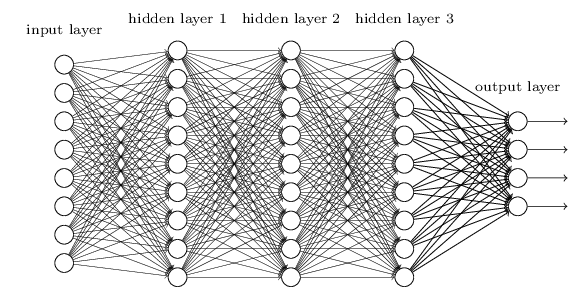
\includegraphics[scale=0.5, width=\linewidth]{figures/Deep_Learning.png}
  \caption{Deep Neural Network}
\end{figure}
\subsection{Convulutional neural networks (CNN's)}
Deep convolutional neural networks or some close variant are used in most neural networks for image recognition problems\cite{?}. They still retain the core concepts of ANN's, such as the way neurons operate and the layered architecture which flows data through the network in order to output a result. However, there are 3 different concepts which distinguish this variant from normal artificial neural networks:
\begin{itemize}
\item Local receptive fields: Each neuron in the first hidden layer will be connected to a small region of the input neurons (called a local receptive field).
\item Shared weights: Weights and biases are shared across the hidden neurons so that convolutional networks become well adapted to translation variances in images. The shared weights and bias are often said to define a kernel or filter. To the map of shared weights from the input layer to the hidden layer we call feature map. A feature detected by a hidden neuron is some kind of input pattern that will cause the neuron to activate. To do image recognition we need more than one feature map in order to recognize multiple features.
\item Pooling layers: Usually are used immediately after convolutional layers. What the pooling layers do is simplify the information in the output from the convolutional layer. A common pool layer is max pooling which provides a way to know if a given feature is found anywhere in a region of the image.\cite{Nielsen2017a} 
\end{itemize}
\subsection{Transfer learning vs learning from scratch}
Supervised learning using deep neural networks requires large amounts of data and computational power in order to train models and determine the network parameters such as weights. However, both of which can either be impossible to have or quite difficult to acquire. Even when one has lots of data and computational power often times the fitting process takes a long time, especially while debugging the network to determine a good model fit.  \par
A common way to solve this problem is the use of a technique called transfer learning. Transfer learning is a method of reusing a model or knowledge for another related task\cite{DipanjanSarkarRaghavBali2018}, in deep learning specifically, it means to carry weights and biases from a generic model trained from a generic dataset like ImageNet which contains 20000 categories like "strawberry" or "balloon" and using those for another model with a different purpose. \par
In CNN's, as inputs are passed along the network hidden layers closer to the input layer output generic features like shapes and curves, while hidden layers closer to the output layers represent more specific categories such as "strawberry" or "balloon" (like the models trained on the ImageNet dataset). Transfer learning aims to obtain parameters from layers that output generic features and build layers on top of those which output specific problem related classes, such as "melanoma" or "nevi". \par
Often times, transfer learning techniques are used to solve image classification problems \cite{Ly2019}, such as the one that we are trying to solve. However, learning from scratch is also an option which can significantly decrease the number of parameters which define the network. To understand why that is, one can think that a lot of parameters in Transfer Learned models are being used to describe features which are not needed for specific problem domains. For instance, if the source model was trained to different foods, it might have learning to indentify its textures. for the and.  Having less parameters means that the model is much smaller compared to transfer learning models (which often reach 100Mb) and can be used on devices such as smartphones which have less computational power.
\subsection{Network Architectures}
Over the years several convolutional neural networks architectures have been developed and tested against state of the art benchmark challenges such as the Imagenet Large Scale Visual Recognition Challenge (ILSVRC) \cite{ilsvrc}. We will describe a few widely used on image classification problems. \par
VGGNet is a network architecture that became quite popular by achieving excellent performance on the ImageNet dataset. There are some public variations of this network, one of which having 16 weight layers (VGG16) that generalizes well onto different datasets, making it a good candidate for our future network. The layers of this architecture are displayed in figure 2.
\begin{figure}[h]
  \centering
    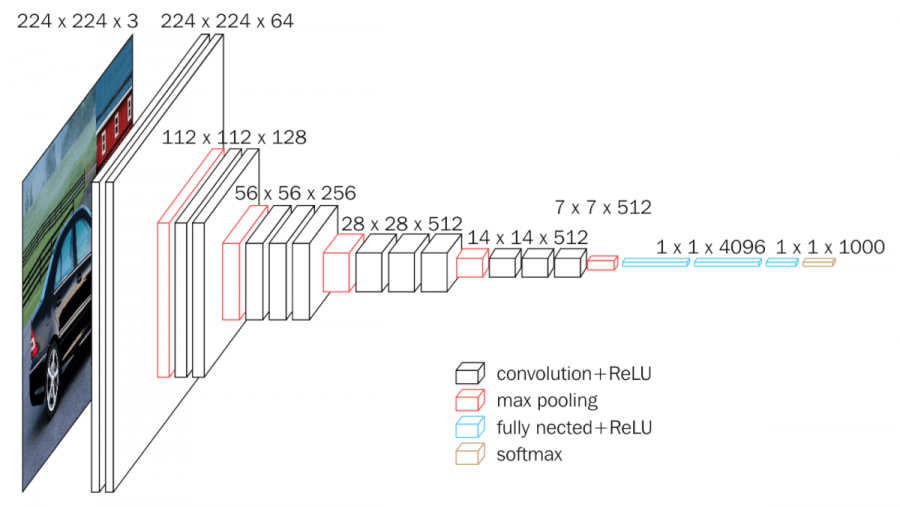
\includegraphics[scale=0.5, width=\linewidth]{figures/vgg16.png}
  \caption{VGG16 Architecture}
\end{figure}
\subsection{Training neural networks}
\subsubsection{Overfitting and underfitting}
The bias and variance trade off is a well known problem in deep learning. The bias of a model is the error caused by the assumptions made to approximate the model to the true predictions. In turn, the variance of a model is an error from sensitivity to small fluctuations in the training set. One must fine tune the model to both accurately make predictions from the training data while generalizing to new data, meaning, we must find a good trade off between bias and variance which minimizes the total error from the model.
If the model underfits then it does not perform well even on the training data, and therefore has high bias and low variance. Simply put, the model doesn't predict well on either training data or new data. However, a common problem while training deep networks is to produce a model that performs well on the training data but that generalizes poorly to any new data \cite{Grus}, such that it starts to either memorize inputs or learn noise. In this case, we say that the model overfits and therefore has low bias but very high variance. \par
In order to evaluate whether a model is underfitting or overfitting one should use state of the art metrics which help describe what is happening while training.  
Multiple solutions to the overfitting problem have been proposed and tested over the years. Methods such as dropout or regularization techniques will certainly help us train our model by reducing complex co-adaptations between neurons, in order to deploy the proposed model into real world use.
\subsubsection{Expanding the training data}
No matter how hard we try to optimize the networks parameters, a model is highly dependent on its dataset. A good dataset is has to:
\begin{itemize}
\item Represent the real world
\item Not be biased, meaning that it favors some classes
\item Be diverse, even if it means that some entries contain noise
\item Contain lots of examples
\end{itemize}
As we've seen there are several datasets available which are labelled for skin lesion diagnosis, however some of them are quite biased towards some specific class or lack large amounts of examples for a specific class. A bad dataset can easily cause the network to overfit because it does not provide enough proper real world examples for the network to produce a good bias variance trade off. As such, when some real world variation is introduced either by noise or some other factor the network fails to predict the class. \par
One way we intent to improve our dataset is through a concept called data augmentation. The main idea behind this concept is to expand the training data by applying operations that reflect real-world variation \cite{Nielsen2017a}, which it turn introduces diversification and size to the dataset.\par 
There is two ways of expanding the training data: 
\begin{itemize}
\item General transformations
\item Generative models
\end{itemize}
We will try to apply both in order to improve our classification accuracy.
\section{Conclusion}
The widespread of the e-Health and m-Health applications along the rise of mobile computing open new opportunities to develop and deploy applications which provide support for patients and health professionals. At the same time, deep learning shows significant improvements in skin lesion diagnosis compared with many other machine learning methods. Even though, there are still challenges to overcome, such as the requirement for large datasets in order to achieve near dermatologist it is expected that these models will continue to improve over the years as more and more data becomes publicly available.



% conference papers do not normally have an appendix

% trigger a \newpage just before the given reference
% number - used to balance the columns on the last page
% adjust value as needed - may need to be readjusted if
% the document is modified later
%\IEEEtriggeratref{8}
% The "triggered" command can be changed if desired:
%\IEEEtriggercmd{\enlargethispage{-5in}}

% references section

% can use a bibliography generated by BibTeX as a .bbl file
% BibTeX documentation can be easily obtained at:
% http://mirror.ctan.org/biblio/bibtex/contrib/doc/
% The IEEEtran BibTeX style support page is at:
% http://www.michaelshell.org/tex/ieeetran/bibtex/
%\bibliographystyle{IEEEtran}
% argument is your BibTeX string definitions and bibliography database(s)
%\bibliography{IEEEabrv,../bib/paper}
%
% <OR> manually copy in the resultant .bbl file
% set second argument of \begin to the number of references
% (used to reserve space for the reference number labels box)

\bibliographystyle{IEEEtran}
\bibliography{Dissertation.bib}
% that's all folks
\end{document}


